\documentclass[conference]{IEEEtran}

\usepackage[colorlinks,linkcolor=blue,filecolor=blue,citecolor=red,bookmarksnumbered=true]{hyperref}
\usepackage{graphicx}
% \usepackage{cite}

\graphicspath{{images/}}

\title{CS239 Project Proposal: Friends Detector}

\author{Alexander~Afanasyev, Chuck Fleming, and Karthikeyan Natarajan \\
% \small \{alexander.afanasyev, tilleyns\}@ucla.edu \\ \\
\small Computer Science Department \\
\small University of California, Los Angeles 
}

\begin{document}

\maketitle

\section{Introduction}

In our project we are going to implement and evaluate the application that detects presence of people faces on a given image or video stream and recognizes (if possible) people names based on previously collected face database. On the high level, our system will consist of five basic components, three of which can be implemented locally and on a remote server (Figure~\ref{fig:basic blocks}): image importer, face database, face detection module, face recognizer module, and visualizer. 

\begin{figure}[htbp]
	\centering
		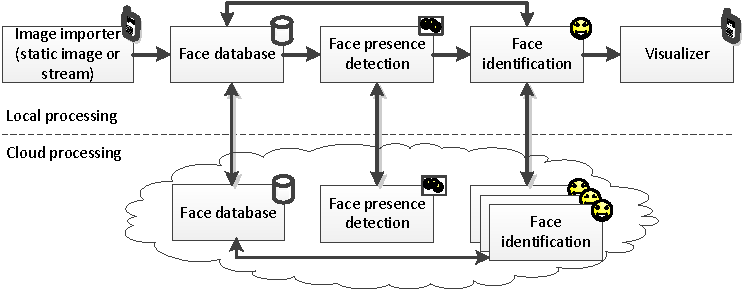
\includegraphics[width=0.6\textwidth]{basic_blocks}
	\caption{Basic blocks of our software}
	\label{fig:basic blocks}
\end{figure}

To provide high fidelity answers the image processing components of our system (the face detection and recognition modules) require a lot of CPU power and memory \emph{{\color{red} For example, detecting presence of face on XXX x YYY image requires YYY seconds and recognizing person using ZZZZZ algorithm agains QQQQ database require WWWWW time.}} At the same time, a lower fidelity answer in the same components can be obtained using coarser granularity (e.g., processing only every 20th image, scaling image before processing) or simpler algorithms (e.g., Eigenfaces algorithm \cite{Turk:1991:Eigenfaces-for-recognition} instead of much more complicated hybrid algorithms \cite{Zhao:2003:Face-recognition:}). 

In mobile environment a dynamic nature of the available resources (e.g., CPU and memory use may be constrained by a user or low battery, network conditions may change any time, etc.) requires the same dynamic view for the class of applications that can provide variable fidelity answers. In other words, an application should maximize fidelity of the answer given resources currently available. In our case with the Friends Detector application we will try to evaluate different combinations of the local and remote face detection and recognition modules and investigate how good faces can be recognized and what are the network, CPU, memory, and battery life requirements in each particular case.

\section{Expected application workflow}

Typical application workflow that we are going to implement:

\begin{itemize}
	\item Selecting picture from the gallery on the phone (1st stage) or selecting camera for image stream capture
	\item For each selected picture or captured frames from the stream:
	\begin{itemize}
		\item Run face detection (local/remote)
		\item For each detected face:
		\begin{itemize}
			\item Run face recognition (local/remote)
			\item Visualize names of recognized people
			\item For every unrecognized person visualize "?" with ability to name person using the context menu and save association in the local/remote database
		\end{itemize}
	\end{itemize}
\end{itemize}

\section{Project timeline}

Our project will be divided in two implementation and one evaluation stage. By the end of the first stage we are expecting to have a working application where we select static images on the mobile phone, process them remotely using simple algorithms, obtain processing result from the remote server, and visualize results on the phone. During the second phase we are going to implement light-weight versions of the image processing components and extend number/quality of algorithms for remote processing.

There several optional components (Facebook, PicasaWeb, and Android contact list photos support in face database) that we may implement if we have enough time.

\subsection{First stage}

Components to be completed:
% Chuck, does openCV have a lot of face recognition algorithms?
% Do they have similar interface?
\begin{center}
\begin{tabular}{|l||l|l|}
	\hline
	\bf Local/remote & \bf Component name & \bf Comment \\
	\hline \hline
	Local & Image importer 	& Static images \\		\hline
	Local & Visualizer 		&  \\       \hline
	Local & Face database	& RPC \\   \hline
	Local & Face detection 	& RPC \\   \hline
	Local & Face recognition & RPC \\  \hline
	Remote & Face database	&  \\     \hline
	Remote & Face detection &  \\     \hline
	Remote & Face recognition & Eigen \\    \hline
	\hline
\end{tabular}
\end{center}


\subsection{Second stage}

Components to be completed:
% Chuck, does openCV have a lot of face recognition algorithms?
% Do they have similar interface?
\begin{center}
\begin{tabular}{|l||l|l|}
	\hline
	\bf Local/remote & \bf Component name & \bf Comment \\
	\hline \hline
	Local & Image importer 	& Video stream \\		\hline
	Local & Face database	& Lightweight \\   \hline
	Local & Face detection 	& Lightweight \\   \hline
	Local & Face recognition & Lightweight \\  \hline
	Remote & Face recognition & openCV algorithms \\    \hline
	% - face identifier
	% 	- Eigen filter, local and remote versions (1st stage)
	% 	- Other models, remote version (2nd stage)
	\hline
\end{tabular}
\end{center}

\subsection{Evaluation}

Evaluation will consist of testing all combinations of local/remote components and different face recognition algorithms within each combination.

\section{Work distribution}

\subsection{First stage}

Alex:
\begin{itemize}
	\item Local visualizer
	\item RPC code for face database, face detection, and face recognition
\end{itemize}

Chuck:
\begin{itemize}
	\item Remote face detection
	\item Remote face database
	\item Remote face recognition (simple algorithm)
\end{itemize}

Karthik:
\begin{itemize}
	\item Application interface design
	\item Local image importer (static images)
	\item Local image preprocessing (e.g., scaling)
\end{itemize}

\subsection{Second stage}

Alex:
\begin{itemize}
	\item Local visualizer (make it work with video stream)
	\item Local face database (lightweight)
	\item Local face detection (lightweight)
	\item Local face recognition (lightweight)
\end{itemize}

Chuck:
\begin{itemize}
	\item Remote face recognition (different algorithms)
\end{itemize}

Karthik:
\begin{itemize}
	\item Local image stream importer
	\item Local image stream preprocessor
\end{itemize}

\subsection{Evaluation}

Every member of our team is going to participate in application evaluation.


\bibliographystyle{IEEEtran}
\bibliography{papers}

\end{document}

% - face manager
% 	- ability to name a person on the photo (1st stage)
% 	- browse the local face database (2nd stage)
% 	- browse the distributed face database (3rd stage)
